\section{Bias and Variance of the Elastic Net Estimator}\label{sec:theory}

Now, assume that \(\mat{X}\) is fixed and that \(\vec{y} = \mat{X}\vec{\beta} +
\vec{\varepsilon}\), where \(\varepsilon_i\) is identically and independently distributed
noise with mean zero and finite variance \(\sigma_\varepsilon^2\). As in the previous
section, we assume that the features are orthogonal. Let \({Z_j} = \tilde{\vec{x}}_j^\T
\vec{y}\) and \(d_j = s_j(\tilde{\vec{x}}_j^\T \tilde{\vec{x}}_j + \lambda_2)\) so that
\(\hat{\beta}_j = \st_{\lambda_1}({Z_j})/d_j\). We can then show that
\begin{equation}
  \label{eq:z-d}
  {Z_j} = \frac{\beta_j^* n \nu_j- \vec{x}_j^\T \vec{\varepsilon}}{s_j}
  \qquad\text{and}\qquad
  d_j = s_j\left(\frac{n \nu_j}{s_j^2} + \lambda_2\right),
\end{equation}
where \(\nu_j\) is the uncorrected sample variance of \(\vec{x}_j\). Please see
\Cref{sec:bias-var-deriv} for a derivation of this and the following results.
Then the bias and variance of \Cref{eq:orthogonal-solution} are given by
\begin{equation*}
  \E \hat\beta_j - \beta_j^* = \frac{1}{d_j}\E \st_\lambda({Z_j}) - \beta^*_j
  \qquad\text{and}\qquad
  \var \hat\beta_j = \frac{1}{d_j^2} \var \st_\lambda({Z_j})
\end{equation*}
where
\begin{equation*}
  \E \st_\lambda({Z_j}) = \int_{-\infty}^{-\lambda}(z + \lambda)f_{Z_j}(z) \du z + \int_{\lambda}^\infty (z - \lambda)f_{Z_j}(z) \du z
\end{equation*}
%
and
\begin{equation}
  \label{eq:st-variance}
  \var {S_\lambda({Z_j})} = \int_{-\infty}^{-\lambda}(z + \lambda)^2f_{Z_j}(z) \du z + \int_{\lambda}^\infty (z - \lambda)^2 f_{Z_j}(z) \du z - \left(\E \st_\lambda({Z_j})\right)^2.
\end{equation}

\subsection{Normally Distributed Noise}

Next, we add the additional assumption that \(\vec{\varepsilon}\) is normally distributed.
Then
\[
  {Z_j} \sim \normal\left(\mu_j = \tilde{\vec{x}}_j^\T\vec{x}_j \beta_j, \sigma_j^2 = \tilde{\vec{x}}_j^\T\tilde{\vec{x}}_j \sigma_\varepsilon^2 \right).
\]
Let \(\theta_j = -\mu_j -\lambda_1 \) and \(\gamma_j = \mu_j - \lambda_1\). Then the
expected value of soft-thresholding of \({Z_j}\) is
\begin{align}
  \E \st_{\lambda_1}({Z_j}) & = \int_{-\infty}^\frac{\theta_j}{\sigma_j} (\sigma_j u - \theta_j) \pdf(u) \du u + \int_{-\frac{\gamma_j}{\sigma_j}}^\infty (\sigma_j u + \gamma_j) \pdf(u) \du u                                               \nonumber                              \\
                            & = -\theta_j \cdf\left(\frac{\theta_j}{\sigma_j}\right) - \sigma_j \pdf\left(\frac{\theta_j}{\sigma_j}\right) + \gamma_j \cdf\left(\frac{\gamma_j}{\sigma_j}\right) + \sigma_j \pdf\left(\frac{\gamma_j}{\sigma_j}\right) \label{eq:mean-centered-eval}
\end{align}
where \(\pdf(u)\) and \(\cdf(u)\) are the probability density and cumulative distribution
functions of the standard normal distribution, respectively. Finally, computing \Cref{eq:st-variance} gives us
\begin{align}
  \label{eq:mean-centered-variance}
  \var{S_\lambda(Z_j)} & = \frac{\sigma_j^2}{2} \left( \erf\left(\frac{\theta_j}{\sigma_j\sqrt{2}}\right) - \frac{\theta_j}{\sigma_j}\sqrt{\frac{2}{\pi}} \exp\left(-\frac{\theta_j^2}{2\sigma_j^2}\right) + 1 \right) + 2 \theta_j \sigma_j \pdf \left(\frac{\theta_j}{\sigma_j}\right) + \theta_j^2 \cdf\left(\frac{\theta_j}{\sigma_j}\right) \nonumber               \\
                       & \phantom{={}} + \frac{\sigma_j^2}{2} \left( \erf\left(\frac{\gamma_j}{\sigma_j\sqrt{2}}\right) - \frac{\gamma_j}{\sigma_j}\sqrt{\frac{2}{\pi}} \exp\left(-\frac{\gamma_j^2}{2\sigma_j^2}\right) + 1 \right) + 2 \gamma_j \sigma_j \pdf \left(\frac{\gamma_j}{\sigma_j}\right) + \gamma_j^2 \cdf\left(\frac{\gamma_j}{\sigma_j}\right) \nonumber \\
                       & \phantom{={}} - \big(\E \st_{\lambda_1}({Z_j})\big)^2.
\end{align}

\subsection{Binary Features}\label{sec:theory-binary-features}

The main focus in this paper is the case when \(\bm{x}_j\) is a binary feature, such that
\(x_{ij} \in \{0, 1\}\) for all \(i\). We define the \emph{class balance} of this feature
as \(q_j = \bar{\bm{x}}_j\): the proportion of ones. For the majority of our results it
would make no difference if we were to swap the ones and zeros as long as an intercept is
included, and ``class balance'' is then equivalent to the proportion of either. But later
on, as we turn to the case of interactions in \Cref{sec:interactions}, we will see that the
choice then matters.

In the case of binary features, inserting \(\nu_j = (q_j - q_j^2)\) (the uncorrected sample
variance for a binary feature) into \Cref{eq:z-d} yields
\[
  {Z_j} = \frac{\beta_j^* n(q_j - q_j^2) - \vec{x}_j^\T \vec{\varepsilon}}{s_j}
  ,\qquad
  d_j = s_j\left(\frac{n(q_j - q_j^2)}{s_j^2} + \lambda_2\right),
\]
% \[
%   \begin{aligned}
%     \tilde{\vec{x}}_j^\T \tilde{\vec{x}}_j & = \frac{1}{s_j^2}(\vec{x}_j - \ones c_j)^\T (\vec{x}_j - \ones c_j) = \frac{1}{s^2_j}(nq - 2nq_j^2 + nq_j^2) = \frac{nq_j(1-q_j)}{s^2_j}, \\
%     \tilde{\vec{x}}_j^\T \vec{x}_j         & = \frac{1}{s_j}(\vec{x}_j^\T \vec{x}_j - \vec{x}_j^\T \ones c_j) = \frac{nq_j(1 - q_j)}{s_j}.
%   \end{aligned}
% \]
and consequently
\[
  \mu_j = \frac{\beta^*_j n(q_j - q_j^2)}{s_j}\qquad \text{and} \qquad \sigma_j^2 = \frac{\sigma_\varepsilon^2n(q_j- q_j^2)}{s^2_j}.
\]
%
We obtain the expected value of the elastic net estimate with respect to \(q_j\) by
inserting \(\mu_j\) and \(\sigma_j\) into \Cref{eq:mean-centered-eval}.

The presence of the factor \(q_j - q_j^2\) in \(\mu_j\), \(\sigma_j^2\), and \(d_j\)
indicates a link between class balance and the elastic net estimator and that this
relationship is mediated by the scaling factor \(s_j\). To achieve some initial intuition
for this relationship, we consider the noiseless case (\(\sigma_\varepsilon = 0\)) in
which, inserting \(\mu_j\) and \(d_j\) into \Cref{eq:orthogonal-solution} yields
\begin{equation}
  \label{eq:noiseless-estimator}
  \hat{\beta}_j = \frac{\st_{\lambda_1}(\tilde{\vec{x}}_j^\intercal \vec{y})}{s_j\left(\tilde{\vec{x}}_j^\intercal \tilde{\vec{x}}_j + \lambda_2\right)}
  =
  \frac{\st_{\lambda_1}\left(\frac{\beta_j^* n (q_j - q_j^2)}{s_j}\right)}{s_j\left(\frac{n(q_j - q_j^2)}{s_j^2} + \lambda_2\right)}.
\end{equation}
%
This expression shows that class balance directly affects the estimator. For values of
\(q_j\) close to \(0\) or \(1\), the input into the soft-thresholding part of the estimator
diminishes and consequently forces the estimate to zero, that is, unless we use the scaling
factor \(s_j = q_j - q_j^2\), in which case the soft-thresholding part will be unaffected
by class imbalance. This choice will not, however, mitigate the impact of class imbalance
on the ridge part of the estimator, for which we would instead need \(s_j = (q_j -
q_j^2)^{1/2}\). For any other choices, \(q_j\) will affect the estimator through both the
ridge and lasso parts, which means that there exists no scaling \(s_j\) that will mitigate
the bias in this case. Later on in \Cref{sec:binary-weighting} we will show how to tackle
this issue for the elastic net by scaling the penalty term individually for each feature.
For now, however, we will continue with the case of normalization.

Based on this reasoning, we will consider the scaling parameterization \(s_j =
(q_j-q_j^2)^\delta\), \(\delta \geq 0\). This includes the cases that we are primarily
interested in, namely \(\delta = 0\) (no scaling), \(\delta = 1/2\) (standard-deviation
scaling), and \(\delta = 1\) (variance scaling). Note that the last of these types,
variance scaling, is not a standard type of normalization; yet, as we have already seen, it
has some interesting properties in the context of binary features.

Another interesting fact about \Cref{eq:noiseless-estimator}, which holds also in the noisy
situation, is that even when the binary feature is balanced (\(q_j = 1/2\)), normalization
will still have an effect on the estimator. Using \(\delta = 0\), for instance, leads the
true coefficient \(\beta_j^*\) in the input to \(\st_\lambda\) to be scaled by \(n (q_j -
q_j^2) = n/4\). For \(\delta = 1\) there would in contrast be no scaling in the
class-balanced case. And for \(\delta = 1/2\), the scaling factor is \(n/2\). Generalizing
this we see that to achieve equivalent scaling in the class-balanced case for all types of
normalization, under our parameterization, we would need to use \(s_j = 4^{\delta - 1} (q_j
- q_j^2)^\delta\). But this only resolves the issue for the lasso. To achieve a similar
effect for ridge regression, we would need another (but similar) modification. Since all
features are binary under our current assumptions we will for now just scale \(\lambda_1\)
and \(\lambda_2\) to account for this effect,\footnote{We use this strategy in all of the
  following examples.} which is equivalent to modifying \(s_j\). We will return to this issue
in \Cref{sec:mixed-data}, when we consider mixes of binary and normal features, in which
case this has significant implications.

We now leave the noiseless scenario and proceed to consider how class balance affects the
bias, variance, and selection probability of the elastic net estimator, starting with the
latter. A consequence of the normal error distribution and consequent normal distribution
of \({Z_j}\) is that the probability of selection in the elastic net problem is given by
\begin{equation}
  \label{eq:selection-probability}
  \Pr\left(\hat{\beta}_j \neq 0\right)
  % & = \Pr\left(\st_{\lambda_1}({Z_j}) \neq 0\right)                                                                                                                                                                                                                           \nonumber \\
  %                                      & = \Pr\left({Z_j} > \lambda_1\right) + \Pr\left({Z_j} < -\lambda_1\right)                                                                                                                                                                                                  \nonumber \\
  %                                      & = \cdf\left(\frac{\mu_j - \lambda_1}{\sigma_j}\right) + \cdf\left(\frac{- \mu_j -\lambda_1}{\sigma_j}\right)                                                                                                                                                              \nonumber \\
  = \cdf \left( \frac{\beta_j^*n (q_j-q_j^2)^{1/2} - \lambda_1(q_j-q_j^2)^{\delta - 1/2}}{\sigma_\varepsilon \sqrt{n}}\right)                 + \cdf \left( \frac{-\beta_j^*n (q_j-q_j^2)^{1/2} - \lambda_1(q_j-q_j^2)^{\delta - 1/2}}{\sigma_\varepsilon \sqrt{n}}\right).
\end{equation}
Letting \(\theta_j = -\mu_j - \lambda_1 \) and \(\gamma_j = \mu_j - \lambda_1\), we can
express this probability asymptotically as \(q_j \rightarrow 1^+\) as
\begin{equation}
  \label{eq:selection-probability-limit}
  \lim_{q_j \rightarrow 1^+} \Pr(\hat{\beta}_j \neq 0) =
  \begin{cases}
    0                                                                & \text{if } 0 \leq \delta < \frac{1}{2}, \\
    2\cdf\left(-\frac{\lambda_1}{\sigma_\varepsilon \sqrt{n}}\right) & \text{if } \delta = \frac{1}{2},        \\
    1                                                                & \text{if } \delta > \frac{1}{2}.
  \end{cases}
\end{equation}

In \Cref{fig:selection-probability}, we plot this probability for various settings of
\(\delta\) for a single feature. Our intuition from the noiseless case holds: suitable
choices of \(\delta\) can mitigate the influence of class imbalance on selection
probability. The lower the value of \(\delta\), the larger the effect of class imbalance
becomes. Note that the probability of selection initially decreases also in the case when
\(\delta \geq 1\). This is a consequence of increased variance of \({Z_j}\) due to the
scaling factor that scales the measurement noise \(\sigma_\varepsilon^2\) upwards. Then, as
\(q_j\) approaches 1, the probability picks up again and eventually approaches 1 for
\(\delta \in \{1, 1.5\}\). The reason for this is that the variance of \({Z_j}\) eventually
explodes (again due to the scaling), which ultimately removes the soft-thresholding effect
altogether. Note that the selection probability is unaffected by \(\lambda_2\).

\begin{figure}[htpb]
  \centering
  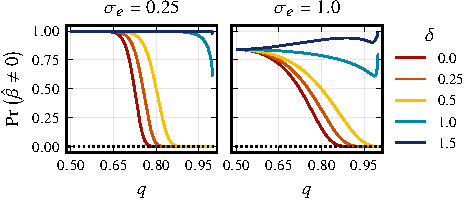
\includegraphics[]{plots/selection_probability.pdf}
  \caption{%
    Probability of selection in the lasso given measurement noise
    % TODO: what is \lambda1 set to here?
    \(\sigma_\varepsilon\), regularization level \(\lambda_1\), and class
    balance \(q\). The scaling factor is set to \(s_j = (q - q^2)^\delta\),
    \(\delta \geq 0\). The dotted line represents the asymptotic limit for
    \(\delta = 1/2\)~(\Cref{eq:selection-probability-limit}).
    \label{fig:selection-probability}}
\end{figure}

Now we turn to the impact of class imbalance on bias and variance of the elastic net
estimator. We begin, in \Cref{thm:classbalance-bias}, by considering the expected value of
the elastic net estimator in the limit as \(q_j \rightarrow 1^+\).

\begin{theorem}
  \label{thm:classbalance-bias}
  If \(\vec{x}_j\) is a binary feature with class balance \(q_j \in (0, 1)\), \(\lambda_1 \in [0,\infty)\), \(\lambda_2 \in [0,\infty)\), \(\sigma_\varepsilon > 0\), and \(s_j = (q_j - q_j^2)^{\delta}\), \(\delta \geq 0\)  then
  \[
    \lim_{q_j \rightarrow 1^+} \E \hat{\beta}_j =
    \begin{cases}
      0                                                                                                  & \text{if } 0 \leq \delta < \frac{1}{2}, \\
      \frac{2n \beta_j^*}{n + \lambda_2} \cdf\left(-\frac{\lambda_1}{\sigma_\varepsilon \sqrt{n}}\right) & \text{if } \delta = \frac{1}{2},        \\
      \beta^*_j                                                                                          & \text{if } \delta > \frac{1}{2}.
    \end{cases}
  \]
\end{theorem}

\Cref{thm:classbalance-bias} shows that the bias of the elastic net estimator approaches
\(-\beta_j^*\) as \(q_j \rightarrow 1^+\) when \(0 \leq \delta < 1/2\). When \(\delta =
1/2\) (standardization), the estimate instead approaches the true coefficient scaled by the
probability that a standard normal variable is smaller than
\(\beta_j^*\sqrt{n}\sigma_\varepsilon^{-1}\). For \(\delta > 1/2\), the estimate is
asymptotically unbiased. This comes as a result of scaling the variance component from the
error term and is accompanied by exponentially increasing variance, which suggests that
variance-scaling may be problematic in the large noise--large imbalance scenario. In
\Cref{thm:classbalance-variance}, we continue by studying the variance in the limit as
\(q_j \rightarrow 1^+\).

\begin{theorem}
  \label{thm:classbalance-variance}
  If \(\vec{x}_j\) is a binary feature with class balance \(q_j \in (0, 1)\) and \(\lambda_1,\lambda_2 \in (0,\infty)\), \(\sigma_\varepsilon > 0\), and \(s_j = (q_j - q_j^2)^{\delta}\), \(\delta \geq 0\), then
  \[
    \lim_{q_j \rightarrow 1^+} \var \hat{\beta}_j =
    \begin{cases}
      0      & \text{if } 0 \leq \delta < \frac{1}{2}, \\
      \infty & \text{if } \delta \geq \frac{1}{2}.
    \end{cases}
  \]
\end{theorem}

\begin{corollary}[Variance in Ridge Regression]
  \label{cor:ridge-variance}
  Assume the conditions of \Cref{thm:classbalance-variance} hold, except that \(\lambda_1 = 0\). Then
  \[
    \lim_{q_j \rightarrow 1^+} \var \hat{\beta}_j =
    \begin{cases}
      0                                          & \text{if } 0 \leq \delta < 1/4, \\
      \frac{\sigma_\varepsilon^2 n}{\lambda_2^2} & \text{if } \delta = 1/4,        \\
      \infty                                     & \text{if } \delta > 1/4.
    \end{cases}
  \]
\end{corollary}

\Cref{thm:classbalance-variance} formally proves the asymptotic variance effects of our
scaling parameter \(s_j\) which we have already discussed in the context of selection
probability and bias. Taken together with the results from \Cref{thm:classbalance-bias},
this suggests that the choice of scaling parameter, at least in the case of our specific
parameterization, introduces a bias--variance tradeoff with respect to \(\delta\): we can
reduce class imbalance-induced bias by increasing \(\delta\) but do so at the price of
increase variance.

In \Cref{fig:bias-var-onedim-lasso}, we now visualize bias, variance, and mean-squared
error for ranges of class balance and various noise-level settings for a lasso problem. The
figure demonstrates the bias--variance tradeoff that our asymptotic results suggest and
indicates that the optimal choice of \(\delta\) is related to the noise level in the data.
Since this level is unknown for most data and can only be estimated in the low-dimensional
setting, it suggests there might be value in selecting \(\delta\) through
hyper-optimization, which we consider in \Cref{sec:experiments-hyperparameter}.\footnote{In
  \Cref{sec:experiments-hyperparameter}, we experiment with this type of hyper-optimization.}
In \Cref{fig:bias-var-onedim-ridge} we show results for ridge regression instead. As
expected, it is \(\delta = 1/2\) that leads to unbiased estimates in this case.

\begin{figure}[htpb]
  \centering
  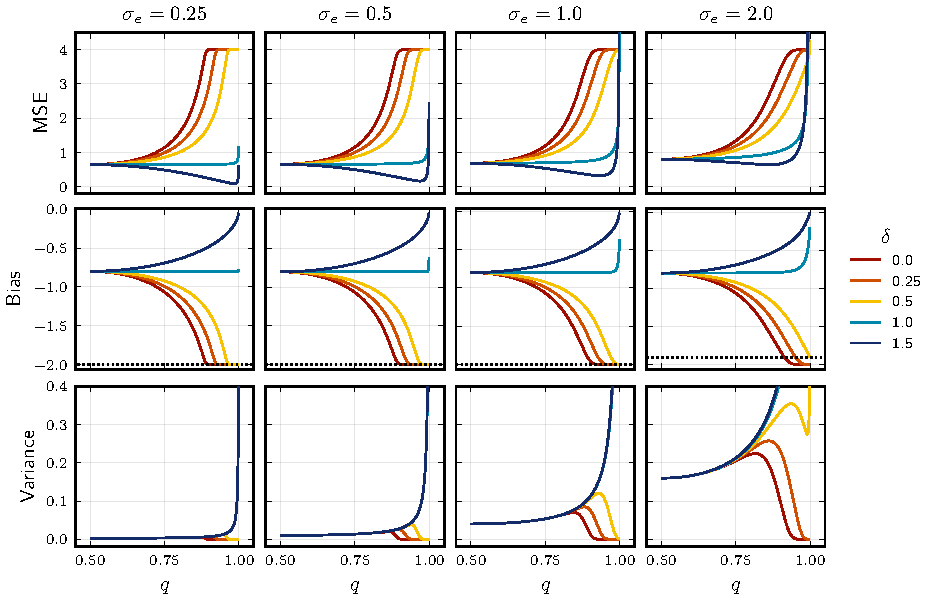
\includegraphics[]{plots/binary_onedim_bias_var_lasso.pdf}
  \caption{%
    Bias, variance, and mean-squared error for a one-dimensional lasso problem,
    parameterized by noise level (\(\sigma_\varepsilon\)), class balance (\(q\)), and
    scaling (\(\delta\)). Dotted lines represent asymptotic bias of the lasso
    estimator in the case when \(\delta = 1/2\).}
  \label{fig:bias-var-onedim-lasso}
\end{figure}

\begin{figure}[htpb]
  \centering
  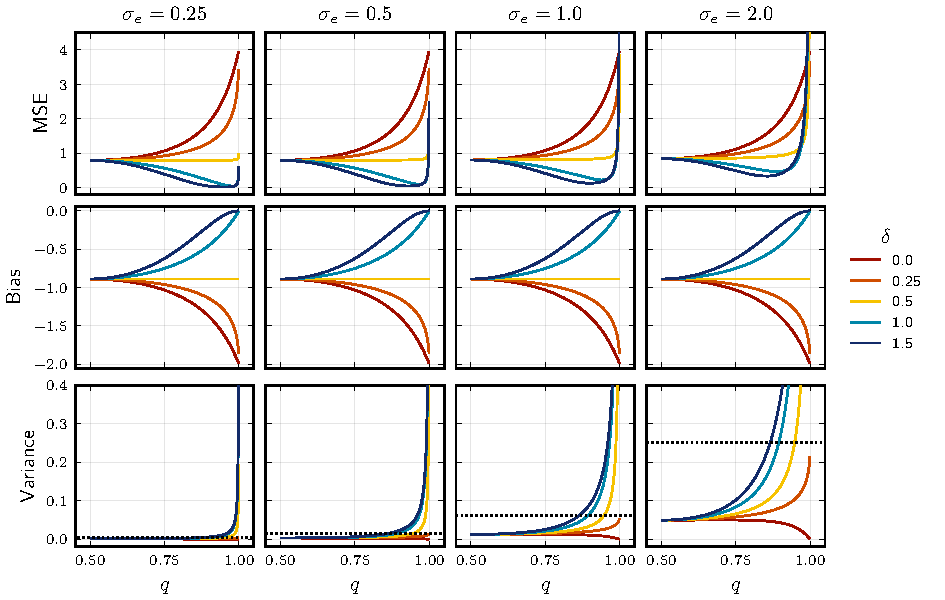
\includegraphics[]{plots/binary_onedim_bias_var_ridge.pdf}
  \caption{%
    Bias, variance, and mean-squared error for one-dimensional ridge regression,
    parameterized by noise level (\(\sigma_\varepsilon\)), class balance (\(q\)), and
    scaling (\(\delta\)). Dotted lines represent asymptotic bias of the ridge
    estimator in the case of \(\delta = 1/4\).}
  \label{fig:bias-var-onedim-ridge}
\end{figure}

% TODO: Consider moving this to the appendix.
So far, we have only considered a single binary feature. But under the assumption of
orthogonal features, it is straightforward to introduce multiple binary features. In a
first example, we study how the power of correctly detecting \(k=10\) signals under \(q_j\)
linearly spaced in \([0.5, 0.99]\)~(\Cref{fig:binary-power}). We set \(\beta^*_j = 2\) for
each of the signals, use \(n = 100\,000\), and let \(\sigma_\varepsilon = 1\). The level of
regularization is set to \(\lambda_1 = n 4^\delta/10\). As we can see, the power is
directly related to \(q_j\) and for unbalanced features stronger the higher the choice of
\(\delta\) is.

We also consider a version of the same setup, but with \(p\) linearly spaced in \([20,
    100]\) and compute normalized mean-squared error (NMSE) and false discovery rate
(FDR)~(\Cref{fig:binary-fdr-mse}). As before, we let \(k = 10\) and consider three
different levels of class imbalance. The remaining \(p-k\) features have class balances
spaced evenly on a logarithmic scale from 0.5 to 0.99. Unsurprisingly, the increase in
power gained from selecting \(\delta = 1\) imposes increased false discovery rates. We also
see that the mean-squared error depends on class balance. In line with our previous
results, \(\delta \in \{0, 1/2\}\) appears to work well for balanced features whilst
\(\delta = 1\) works better when there are large imbalances. In the case when \(q_j =
0.99\), the model under scaling with \(\delta = 0\) does not detect any of the true
signals.

\begin{figure}[htpb]
  \centering
  \subcaptionbox{%
    The power (probability of detecting all true signals) of the lasso. In our orthogonal
    setting, power is constant over \(p\), which is why we have omitted the parameter in the
    plot. \label{fig:binary-power}
  }{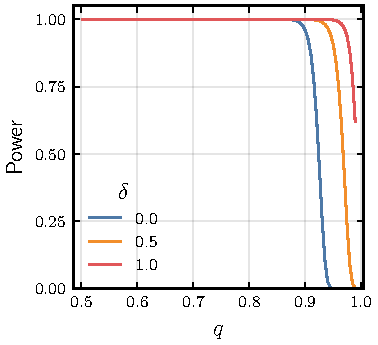
\includegraphics[]{plots/power.pdf}}\hfill%
  \subcaptionbox{%
    NMSE and FDR: the rate of coefficients incorrectly set to non-zero (false discoveries) to
    the total number of estimated coefficients that are nonzero (discoveries).
    \label{fig:binary-fdr-mse} }{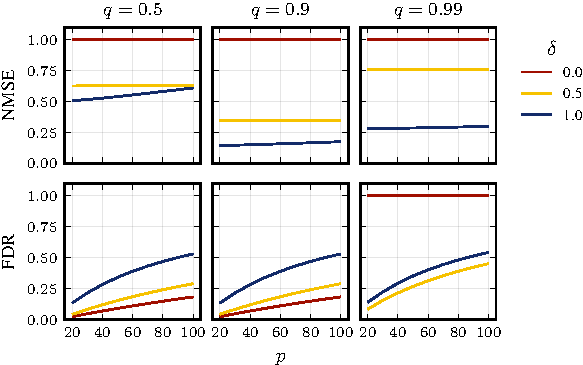
\includegraphics[]{plots/fdr_mse.pdf}}%%
  % 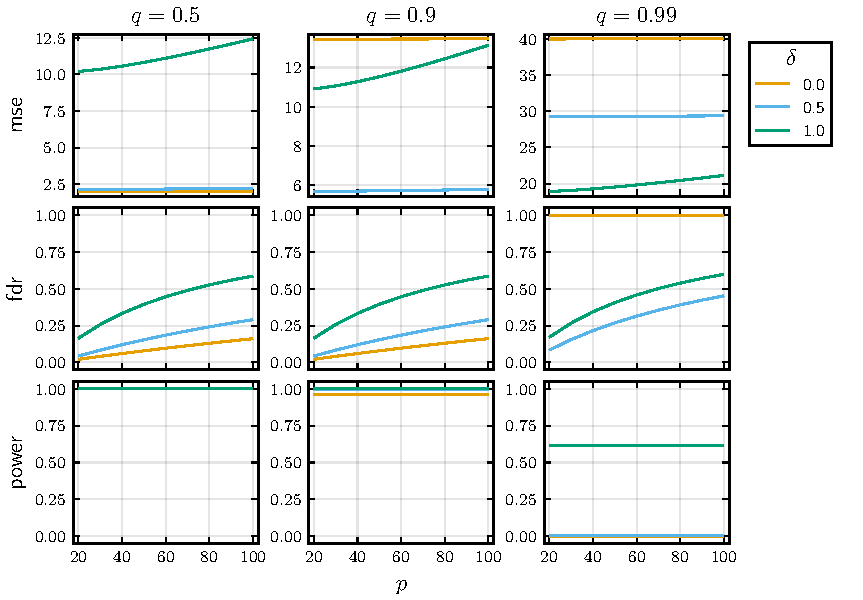
\includegraphics[]{plots/beta-bias-multidim.pdf}
  \caption{%
    Normalized mean-squared error (NMSE), false discovery rate (FDR), and power for a lasso problem with
    \(k = 10\) true signals (nonzero \(\beta_j^*\)), varying \(p\), and \(q_j \in [0.5, 0.99]\). The noise level is set at \(\sigma_\varepsilon = 1\) and \(\lambda_1 = 0.02\).
  }
\end{figure}

In \Cref{sec:experiments}, we will continue to study binary features in simulated
experiments. For now, however, we turn to the case of mixed data.

\subsection{Mixed Data}\label{sec:mixed-data}

In this section we consider the case where features are made up of a mix of continuous and
binary features. Throughout the section we continue to assume that \(\mat{X}\) is fixed and
that the features are orthogonal to one another and restrict our scope to the case where
the continuous features are normally distributed.

A fundamental problem with mixed data is deciding how to put binary and normal features on
the same scale in order to regularize each type of feature fairly. In principle we need to
match a one-unit change in the binary feature with some amount of change in the normal
feature. To setup this situation formally, we will say that the effects of a binary feature
\(\vec{x}_1\) and a normal feature \(\vec{x}_2\) are \emph{comparable} if \(\beta^*_1 =
\kappa \sigma \beta^*_2\), where \(\kappa > 0\) represents the number of standard
deviations of the normal feature we consider to be comparable to one unit on the binary
feature. We illustrate this notion of comparability by the following examples.

% TODO: illustrate this with a figure
\begin{example}
  Assume \(\kappa = 2\). If \(\vec{x}_2\) is sampled from
  \(\normal\left(\mu_j, \sigma^2 = (1/2)^2\right)\), then the effects of \(\vec{x}_1\) and
  \(\vec{x}_2\) are comparable if \(\beta_1^* = 2\sigma \beta_2^* = \beta_2^*\).
\end{example}
\begin{example}
  Assume \(\kappa = 1\). If \(\vec{x}_2\) is sampled from \(\normal(\mu,
  \sigma^2 = 2^2)\), then the effects of \(\vec{x}_1\) and \(\vec{x}_2\) are comparable if
  \(\beta_1^* = \sigma\beta_2^* = 2\beta_2^*\).
\end{example}

The definition above refers to the true coefficients, but for our regularized estimates we
want \(\hat{\beta}_1 = \kappa\sigma\hat{\beta}_2\) to hold. If we assume that we are in a
noiseless situation (\(\sigma_\varepsilon = 0\), are standardizing the normal feature and
that, and that, for simplicity, \(\bm{x}_1\) has mean zero, then we need the following
equality to hold:
%
\begin{equation}
  \label{eq:comparable-effects}
  \hat{\beta}_1 = \frac{\st_{\lambda_1}(\tilde{\vec{x}}_1^\intercal \vec{y})}{s_1\left(\tilde{\vec{x}}_1^\intercal \tilde{\vec{x}}_1 + \lambda_2\right)}
  = \frac{\st_{\lambda_1}\left(\frac{n\beta_1^* (q - q^2)}{s_1}\right)}{s_1\left(\frac{n(q - q^2)}{s_1^2} + \lambda_2\right)}
  = \frac{\kappa\sigma \st_{\lambda_1}(\tilde{\vec{x}}_2^\intercal \vec{y})}{s_2\left(\tilde{\vec{x}}_2^\intercal \tilde{\vec{x}}_2 + \lambda_2\right)}
  = \frac{\kappa \st_{\lambda_1}\left(\frac{n\beta_1^*}{\kappa} \right)}{n + \lambda_2}
  = \kappa \hat{\beta}_2.
\end{equation}
%
For the lasso (\(\lambda_2 = 0\)) and ridge regression (\(\lambda_1=0\)), we see that the
equation holds for \(s_1 = \kappa (q - q^2)\) and \(s_1 = (q - q^2)^{1/2}\), respectively.
In other words, we achieve comparability in the lasso by scaling each binary feature with
its variance times \(\kappa\). And for ridge regression, we can achieve comparability by
scaling with standard deviation, irrespective of \(\kappa\). For any other choices of
\(s_1\), equality holds only at a single fixed level of class balance. Let this level be
\(q_0\). Then, to achieve equality for \(\lambda_2 = 0\), we need \(s_1 =\kappa (q_0 -
q_0^2)^{1 - \delta}(q - q^2)^\delta\). Similarly, for \(\lambda_1 = 0\), we need \(s_1 =
(q_0 - q_0^2)^{1 - 2\delta} (q - q^2)^\delta\). In the sequel, we will assume that \(q_0 =
1/2\), to have effects be equivalent for the class-balanced case.

Note that this means that the choice of normalization has an implicit effect on the
relative penalization of binary and normal features, even in the class-balanced case (\(q_1
= 1/2\)). If we for instance use \(\delta=0\) and fit the lasso, then
\Cref{eq:comparable-effects} for a binary feature with \(q_1=1/2\) becomes
\(4\st_{\lambda_1}\left(n\beta_1^*/4\right) = \kappa \st_{\lambda_1}(n\beta_1^*/\kappa ),\)
which implies \(\kappa = 4\). In other words, the choice of normalization equips our model
with a belief about how binary and normal features should be penalized relative to one
another.

For the rest of this paper, we will use \(\kappa = 2\) and say that the effects are
comparable if the effect of a flip in the binary feature equals the effect of a
two-standard deviation change in the normal feature. We motivate this choice by an argument
of \citet{gelman2008}, who suggests that the classical use of standardized regression
coefficients to compare effects in a regression model is a default that unduly emphasizes
effects of continuous features for many real data sets. We want to stress that the choice
of \(\kappa\) should if possible be based on contextual knowledge of the data and that our
results depend only superficially on this particular setting. We do, however, want to
emphasize that this choice should be made \emph{actively} and not be allowed to implicitly
depend on the type of normalization used.

Finally, note that we assumed a noiseless case above. In the presence of noise, the bias
induced by the combination of noise level and normalization choice will affect these
results (see \Cref{fig:bias-var-onedim-lasso}), which means that normally distributed and
binary features will not be comparable in this case.

\subsection{Interactions}\label{sec:interactions}

The elastic net can be extended to include interactions. There is previous literature on
this topic~\citep{bien2013,zemlianskaia2022,lim2015}, but it has not considered the
possible influence of normalization. Here, we will consider simple pairwise interactions
with no restriction on the presence of main effects. For our analysis, we let \(\vec{x}_1\)
and \(\vec{x}_2\) be two features of the data and \(\bm{x}_3\) their interaction. Our model
is \(\bm{y}=\beta_0 + \bm{X\beta} + \bm{\varepsilon}\) as before, with \(\beta_3\)
representing the effect of the interaction.

We consider two cases in which we assume that the features are orthogonal and that
\(\vec{x}_1\) is binary with class balance \(q_1\). In the first case, we let \(\bm{x}_2\)
be normal with mean \(\mu\) and variance \(\sigma^2\), and in the second case \(\bm{x}_2\)
be binary with class balance \(q_2\). To construct the interaction feature, we center the
main features and then multiply element-wise. The elements of the interaction feature are
then given by \(x_{3,i} = (x_{1,i} - \bar{\bm{x}}_1)(x_{2,i} - \bar{\bm{x}}_2)\). The main
motivation for centering is that it removes correlation between the main features and the
interaction, which would otherwise affect the estimates due to the regularization. The oth

Centering normal features is also important because it ensures that their means do not
factor into the estimation of their effects, which is otherwise the case since the variance
of \(\bm{x}_3\) would then be \(q_1(\sigma^2 + \mu^2(1 - q_1))\) in the case when
\(\bm{x}_1\) is centered and \((q_1 - q_1^2)(\sigma^2 + \mu^2)\) otherwise. Centering
binary features is also important because the variance of the interaction term is otherwise
\(q_1\sigma^2\) (provided \(\bm{x}_2\) is centered), which would mean that the
encoding\footnote{Whether values are \{0,1\} or \{-1, 1\} for instance.} of values of the
binary feature would directly affect the interaction term.

If \(\bm{x}_2\) is normal and both features are centered before computing the interaction
term, the variance becomes \(\sigma^2 (q-q^2)\), which suggests using \(s_3 = \sigma (q -
q^2)^\delta\) along the lines of our previous reasoning. And if \(\bm{x}_2\) is binary,
instead, then similar reasoning suggests using \(s_3 = ((q_1-q_1^2)(q_2-q_2^2))^\delta\).
In \Cref{sec:experiments-interactions}, we will study the effects of these choices in
simulated experiments.

\subsection{The Weighted Elastic Net}\label{sec:binary-weighting}

We have so far shown that certain choices of normalization can mitigate the class-balance
bias imposed by the lasso and ridge regularization. But we have also
demonstrated~(\Cref{sec:theory-binary-features}) that there is no (simple) choice of
scaling that can achieve the same effect for the elastic net.
\Cref{eq:noiseless-estimator}, however, suggests a natural alternative to normalization,
which is to use the weighted elastic net~(\Cref{sec:weighted-elasticnet}). We can then
control class-balance bias by setting our weights according to \(u_j = v_j = (q_j -
q_j^2)^{\omega}\) and counteract it, at least in the noiseless case, with \(\omega = 1\).
For the lasso and ridge regression, this is equivalent to using \(\delta = 1\) and \(\delta
= 1/2\) respectively.

Results analogous to those in \Cref{sec:theory-binary-features} can be attained with a few
small modifications for the weighted elastic net case. Starting with selection probability,
we can set \(s_j = 1\) and replace \(\lambda_1\) with \(\lambda_1 u_j =
\lambda_1(q_j-q_j^2)^\omega\) in \Cref{eq:selection-probability}, which shows that
\(\omega\) and \(\delta\) have interchangeable effects for selection probability. Note that
this extends to the limit in \Cref{eq:selection-probability-limit}.

As far as expected value and variance of the weighted elastic net estimator is concerned,
the quantities in \Cref{eq:mean-centered-eval} and \Cref{eq:mean-centered-variance} apply
directly in the case of the weighted elastic net given \(s_j = 1\) for all \(j\) and
replacing \(\lambda_1\) as in the previous paragraph and \(\lambda_2\) with \(\lambda_2
(q_j - q_j^2)^\omega\). On the other hand, the asymptotic results differ slightly as we
will show next, starting with the expected value.

\begin{theorem}
  \label{thm:weighted-elasticnet-bias}
  Let \(\vec{x}_j\) be a binary feature with class balance \(q_j \in (0, 1)\) and take
  \(\lambda_1 > 0\), \(\lambda_2 > 0\), and \(\sigma_\varepsilon > 0\). For the
  weighted elastic net with weights \(u_j = v_j = (q_j-q_j^2)^\omega\) and \(\omega \geq 0\), it holds that
  \[
    \lim_{q_j \rightarrow 1^+} \E \hat{\beta}_j =
    \begin{cases}
      0                              & \text{if } 0 \leq \omega < 1, \\
      \frac{\beta^*n}{n + \lambda_2} & \text{if } \omega = 1,        \\
      \beta^*                        & \text{if } \omega > 1.
    \end{cases}
  \]
\end{theorem}

This result is similar to the one for the unweighted but normalized elastic net. The only
difference arises in the case when \(\omega = 1\), in which case the limit is unaffected by
\(\lambda_1\) in the case of the weighted elastic net.

\begin{theorem}
  \label{thm:weighted-elasticnet-variance}
  Let \(\vec{x}_j\) be a binary feature with class balance \(q_j \in (0, 1)\) and take
  \(\lambda_1 > 0\), \(\lambda_2 > 0\), and \(\sigma_\varepsilon > 0\). For the
  weighted elastic net with weights \(u_j = v_j = (q_j-q_j^2)^\omega\) and \(\omega \geq 0\), it holds that
  \[
    \lim_{q_j \rightarrow 1^+} \var \hat{\beta}_j =
    \begin{cases}
      0      & \text{if } 0 \leq \delta < \frac{1}{2}, \\
      \infty & \text{if } \delta \geq \frac{1}{2}.
    \end{cases}
  \]
\end{theorem}

This result mimics the result for asymptotic variance in the case of the unweighted elastic
net with normalization. In \Cref{fig:binary-onedim-bias-var-elnet}, we plot bias, variance,
and mean-squared error for the weighted elastic net. Again, we see that the behavior of
bias as \(q_j \rightarrow 1^+\) depends on noise level and that there is a bias--variance
tradeoff with respect to \(\omega\). As in \Cref{sec:mixed-data}, we modify the weighting
factor to have comparability under \(\kappa = 2\).

\begin{figure}[htpb]
  \centering
  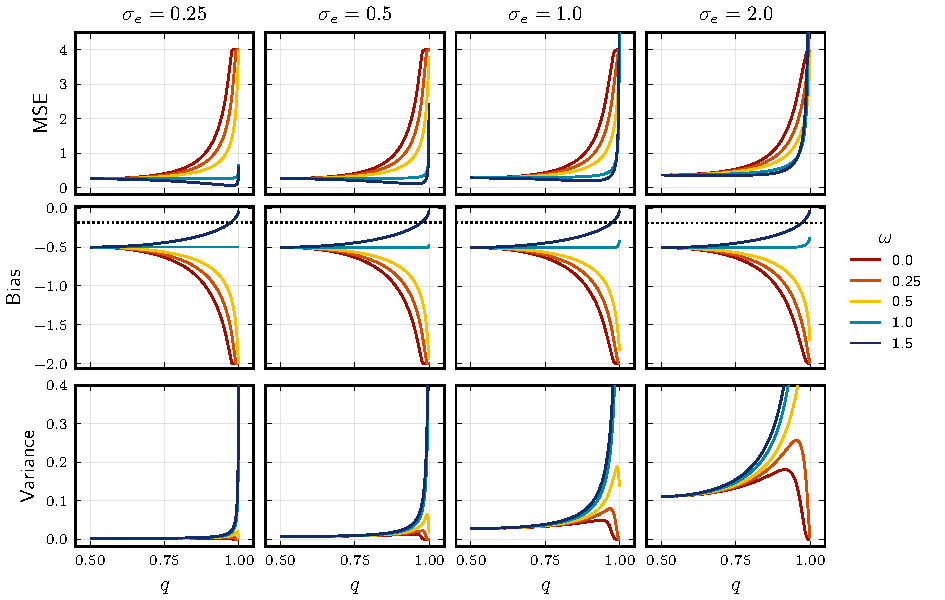
\includegraphics[]{plots/binary_onedim_bias_var_elnet.pdf}
  \caption{%
    Bias, variance, and mean-squared error in the case of the one-dimensional weighted elastic
    net. The measures are shown for different noise levels (\(\sigma_\varepsilon\)), class
    balances (\(q_j\)), and values of (\(\omega\)), which controls the weights that are set to
    \(u_j = v_j = 2\times 4^{\omega - 1}(q-q^2)^\omega\) in order for the results to be
    comparable across different values of \(\omega\). The dotted lines represent the asymptotic
    bias of the estimator in the case of \(\omega = 1\). In the case of \(\omega > 1\), the
    limit of the bias is zero. \label{fig:binary-onedim-bias-var-elnet}
  }
\end{figure}
